\documentclass[11pt]{article}
\usepackage[textwidth=18.0cm, textheight=23.0cm, top=2.0cm]{geometry}
\usepackage{pst-all}
\usepackage{amssymb}
\usepackage{tikz}
\usepackage{underscore}\begin{document}
\pagestyle{empty}


ClassName: \underline{\textbf{Class_03.2bp-27}}
\par
BinSize: \underline{\textbf{40 × 40}}
\par
ReduceSize: \underline{\textbf{40 × 40}}
\par
TypeNum: \underline{\textbf{58}}
\par
Num: \underline{\textbf{60}}
\par
OutS: \underline{\textbf{24000}}
\par
InS: \underline{\textbf{20453}}
\par
Rate: \underline{\textbf{0.852}}
\par
UB: \underline{\textbf{15}}
\par
LB0: \underline{\textbf{15}}
\par
LB: \underline{\textbf{15}}
\par
LBWithCut: \underline{\textbf{15}}
\par
NodeCut: \underline{\textbf{0}}
\par
ExtendedNodeCnt: \underline{\textbf{1}}
\par
GenNodeCnt: \underline{\textbf{1}}
\par
PrimalNode: \underline{\textbf{0}}
\par
ColumnCount: \underline{\textbf{15}}
\par
TotalCutCount: \underline{\textbf{0}}
\par
RootCutCount: \underline{\textbf{0}}
\par
LPSolverCnt: \underline{\textbf{1}}
\par
PricingSolverCnt: \underline{\textbf{0}}
\par
BranchAndBoundNum: \underline{\textbf{1}}
\par
isOpt: \underline{\textbf{true}}
\par
TimeOnInitSolution: \underline{\textbf{600.000 s}}
\par
TimeOnPrimal: \underline{\textbf{0.000 s}}
\par
TimeOnPricing: \underline{\textbf{0.000 s}}
\par
TimeOnRmp: \underline{\textbf{0.062 s}}
\par
TotalTime: \underline{\textbf{600.375 s}}
\par
\newpage


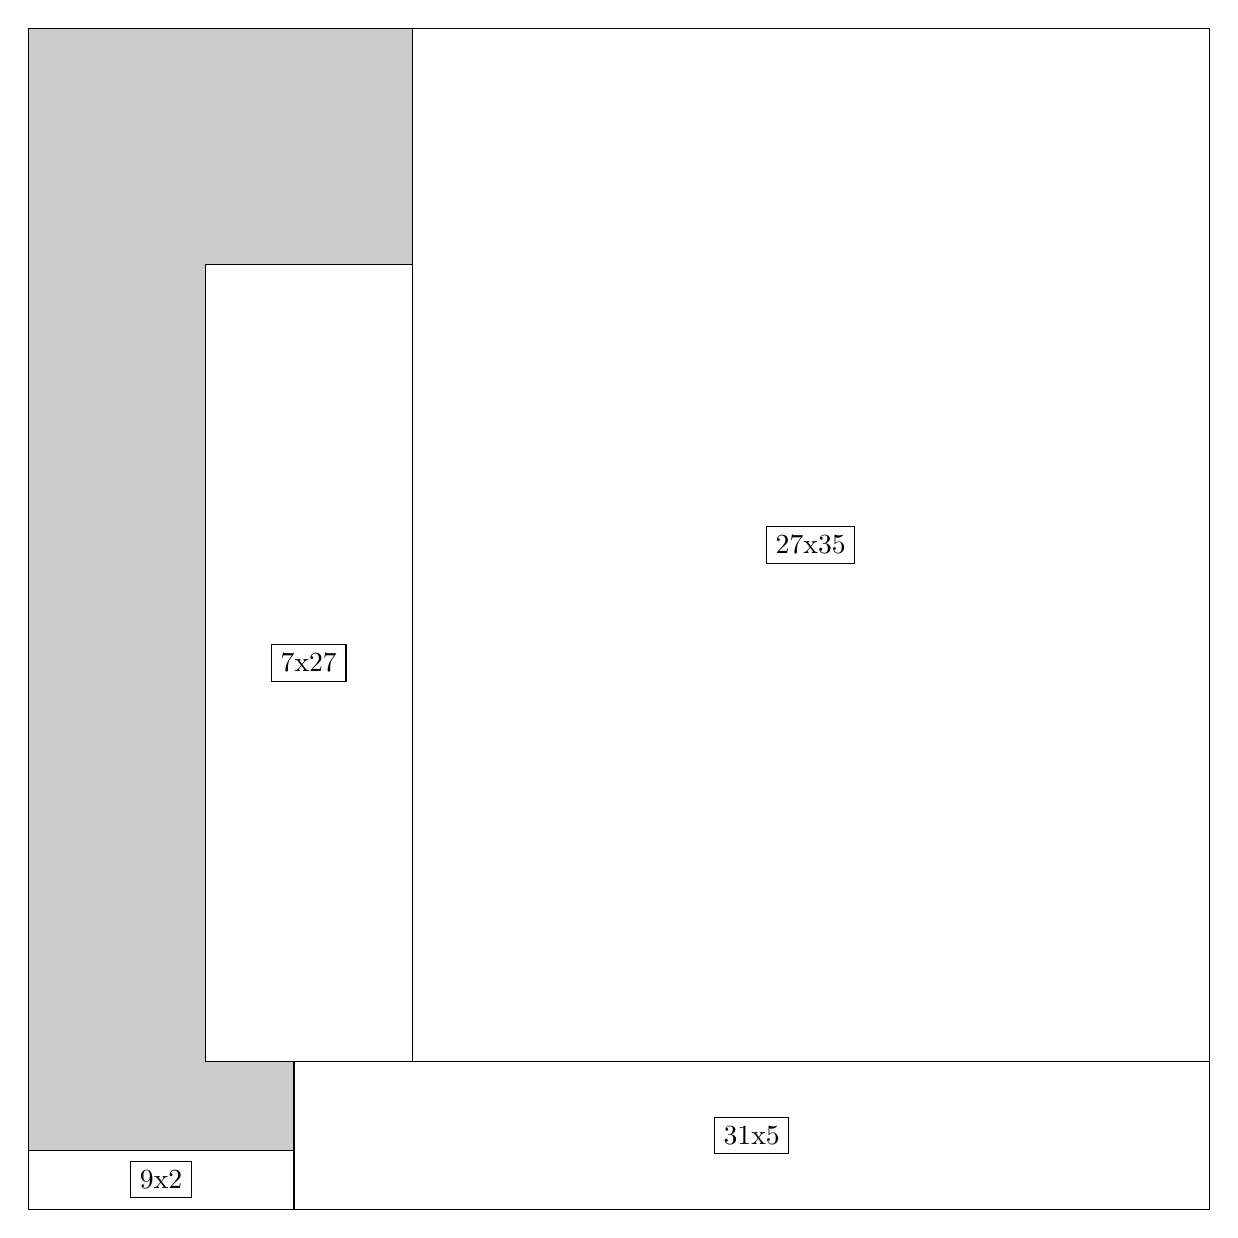
\begin{tikzpicture}[shorten >=1pt,scale=1.0,every node/.style={scale=1.0},->]
\tikzstyle{vertex}=[circle,fill=black!25,minimum size=14pt,inner sep=0pt]
\filldraw[fill=gray!40!white, draw=black] (0,0) rectangle (15.0,15.0);
\foreach \name/\x/\y/\w/\h in {31x5/3.375/0.0/11.625/1.875,9x2/0.0/0.0/3.375/0.75,27x35/4.875/1.875/10.125/13.125,7x27/2.25/1.875/2.625/10.125}
\filldraw[fill=white!40!white, draw=black] (\x,\y) rectangle node[draw] (\name) {\name} ++(\w,\h);
\end{tikzpicture}


w =31 , h =5 , x =9 , y =0 , v =155
\par
w =9 , h =2 , x =0 , y =0 , v =18
\par
w =27 , h =35 , x =13 , y =5 , v =945
\par
w =7 , h =27 , x =6 , y =5 , v =189
\par
\newpage


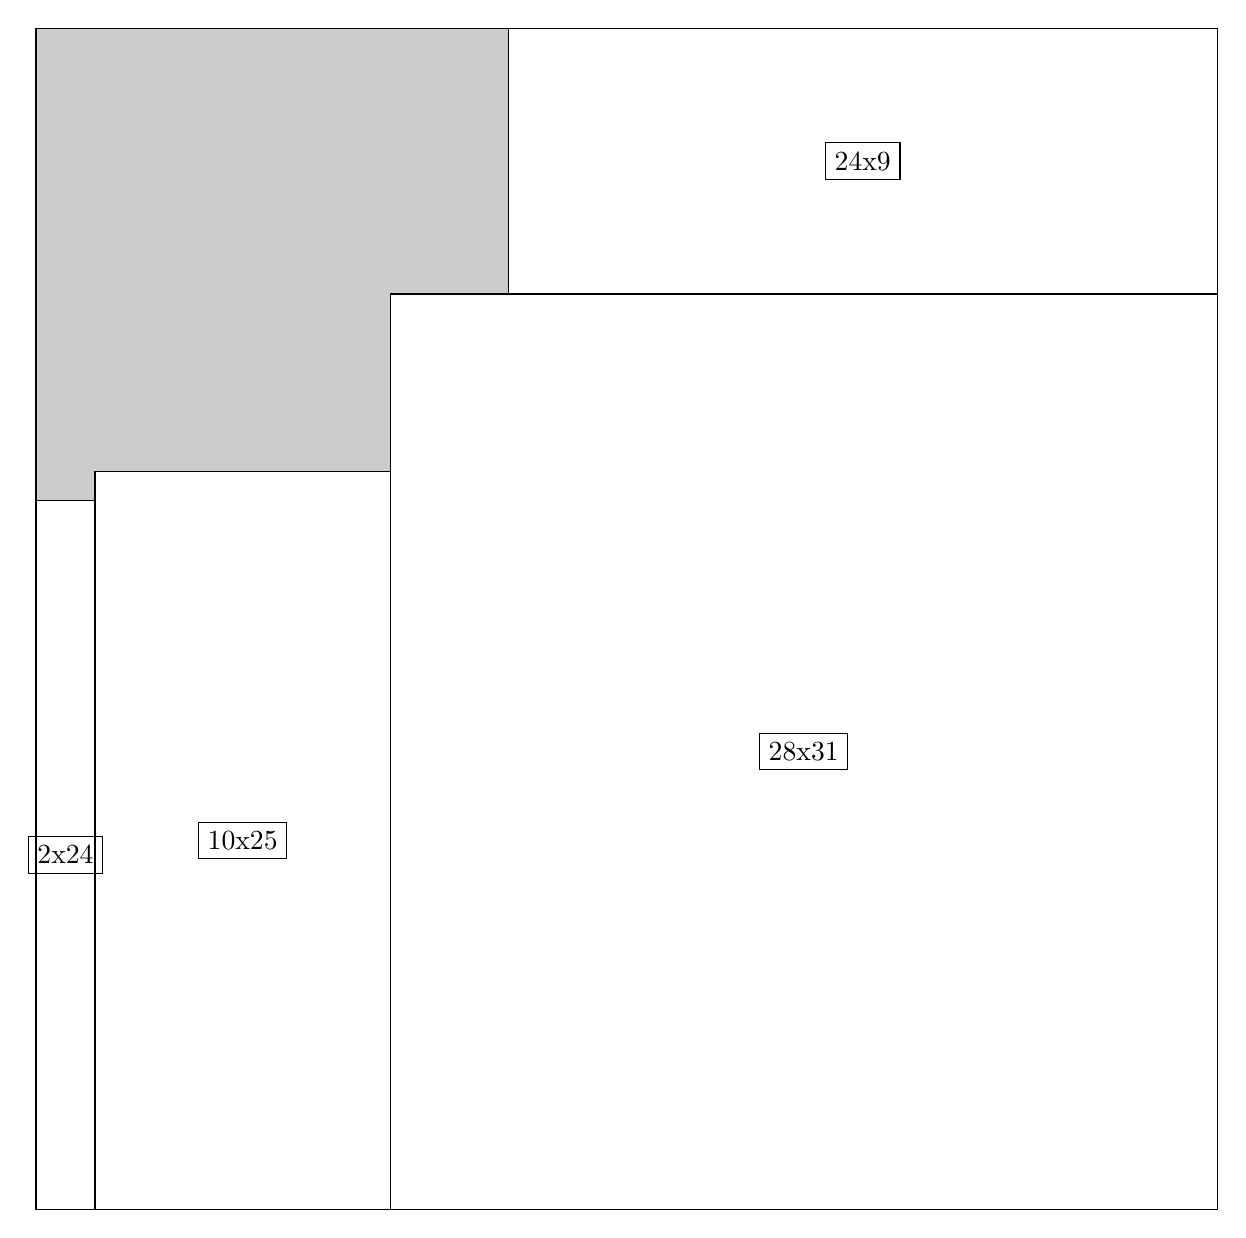
\begin{tikzpicture}[shorten >=1pt,scale=1.0,every node/.style={scale=1.0},->]
\tikzstyle{vertex}=[circle,fill=black!25,minimum size=14pt,inner sep=0pt]
\filldraw[fill=gray!40!white, draw=black] (0,0) rectangle (15.0,15.0);
\foreach \name/\x/\y/\w/\h in {28x31/4.5/0.0/10.5/11.625,24x9/6.0/11.625/9.0/3.375,10x25/0.75/0.0/3.75/9.375,2x24/0.0/0.0/0.75/9.0}
\filldraw[fill=white!40!white, draw=black] (\x,\y) rectangle node[draw] (\name) {\name} ++(\w,\h);
\end{tikzpicture}


w =28 , h =31 , x =12 , y =0 , v =868
\par
w =24 , h =9 , x =16 , y =31 , v =216
\par
w =10 , h =25 , x =2 , y =0 , v =250
\par
w =2 , h =24 , x =0 , y =0 , v =48
\par
\newpage


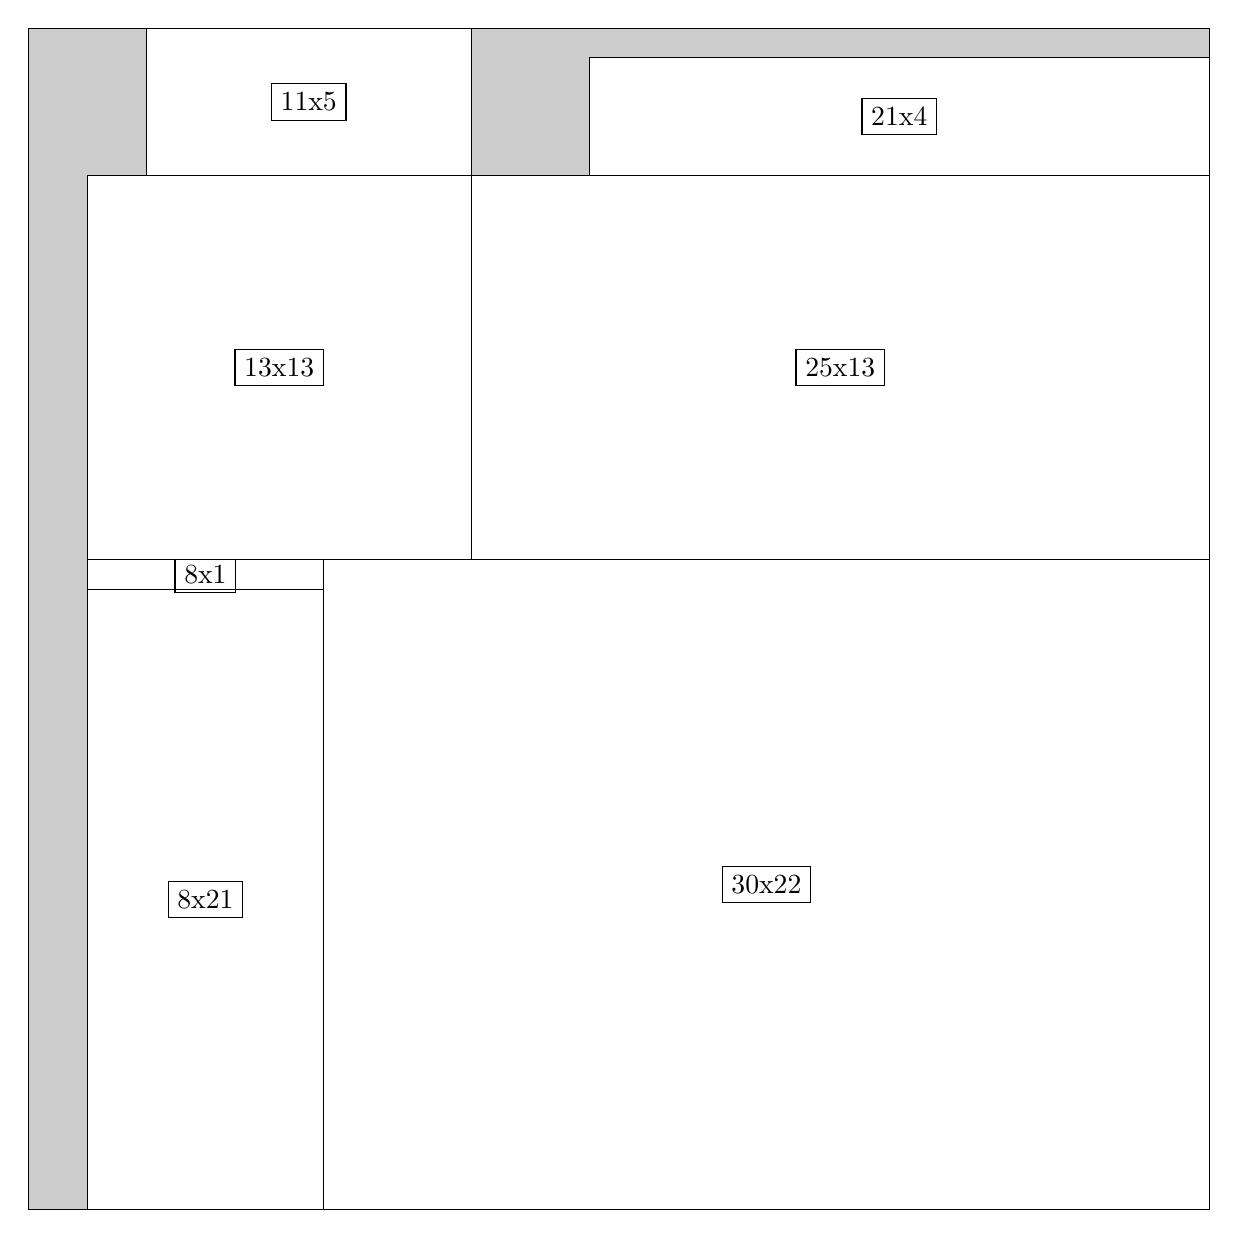
\begin{tikzpicture}[shorten >=1pt,scale=1.0,every node/.style={scale=1.0},->]
\tikzstyle{vertex}=[circle,fill=black!25,minimum size=14pt,inner sep=0pt]
\filldraw[fill=gray!40!white, draw=black] (0,0) rectangle (15.0,15.0);
\foreach \name/\x/\y/\w/\h in {30x22/3.75/0.0/11.25/8.25,8x21/0.75/0.0/3.0/7.875,8x1/0.75/7.875/3.0/0.375,25x13/5.625/8.25/9.375/4.875,21x4/7.125/13.125/7.875/1.5,13x13/0.75/8.25/4.875/4.875,11x5/1.5/13.125/4.125/1.875}
\filldraw[fill=white!40!white, draw=black] (\x,\y) rectangle node[draw] (\name) {\name} ++(\w,\h);
\end{tikzpicture}


w =30 , h =22 , x =10 , y =0 , v =660
\par
w =8 , h =21 , x =2 , y =0 , v =168
\par
w =8 , h =1 , x =2 , y =21 , v =8
\par
w =25 , h =13 , x =15 , y =22 , v =325
\par
w =21 , h =4 , x =19 , y =35 , v =84
\par
w =13 , h =13 , x =2 , y =22 , v =169
\par
w =11 , h =5 , x =4 , y =35 , v =55
\par
\newpage


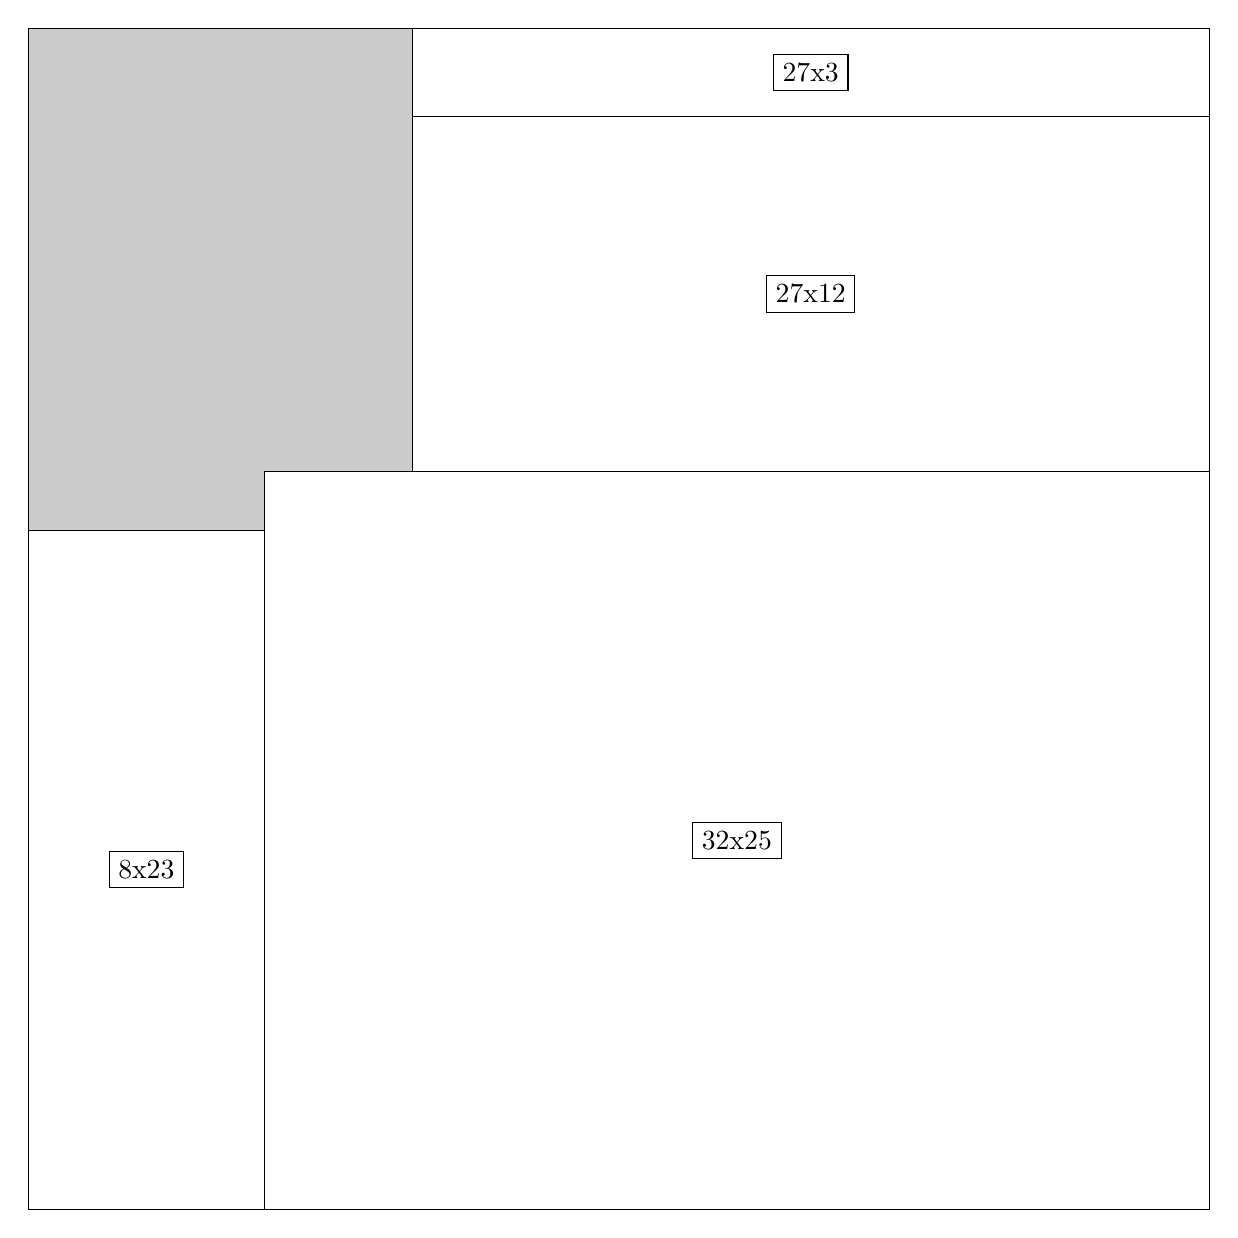
\begin{tikzpicture}[shorten >=1pt,scale=1.0,every node/.style={scale=1.0},->]
\tikzstyle{vertex}=[circle,fill=black!25,minimum size=14pt,inner sep=0pt]
\filldraw[fill=gray!40!white, draw=black] (0,0) rectangle (15.0,15.0);
\foreach \name/\x/\y/\w/\h in {32x25/3.0/0.0/12.0/9.375,27x12/4.875/9.375/10.125/4.5,27x3/4.875/13.875/10.125/1.125,8x23/0.0/0.0/3.0/8.625}
\filldraw[fill=white!40!white, draw=black] (\x,\y) rectangle node[draw] (\name) {\name} ++(\w,\h);
\end{tikzpicture}


w =32 , h =25 , x =8 , y =0 , v =800
\par
w =27 , h =12 , x =13 , y =25 , v =324
\par
w =27 , h =3 , x =13 , y =37 , v =81
\par
w =8 , h =23 , x =0 , y =0 , v =184
\par
\newpage


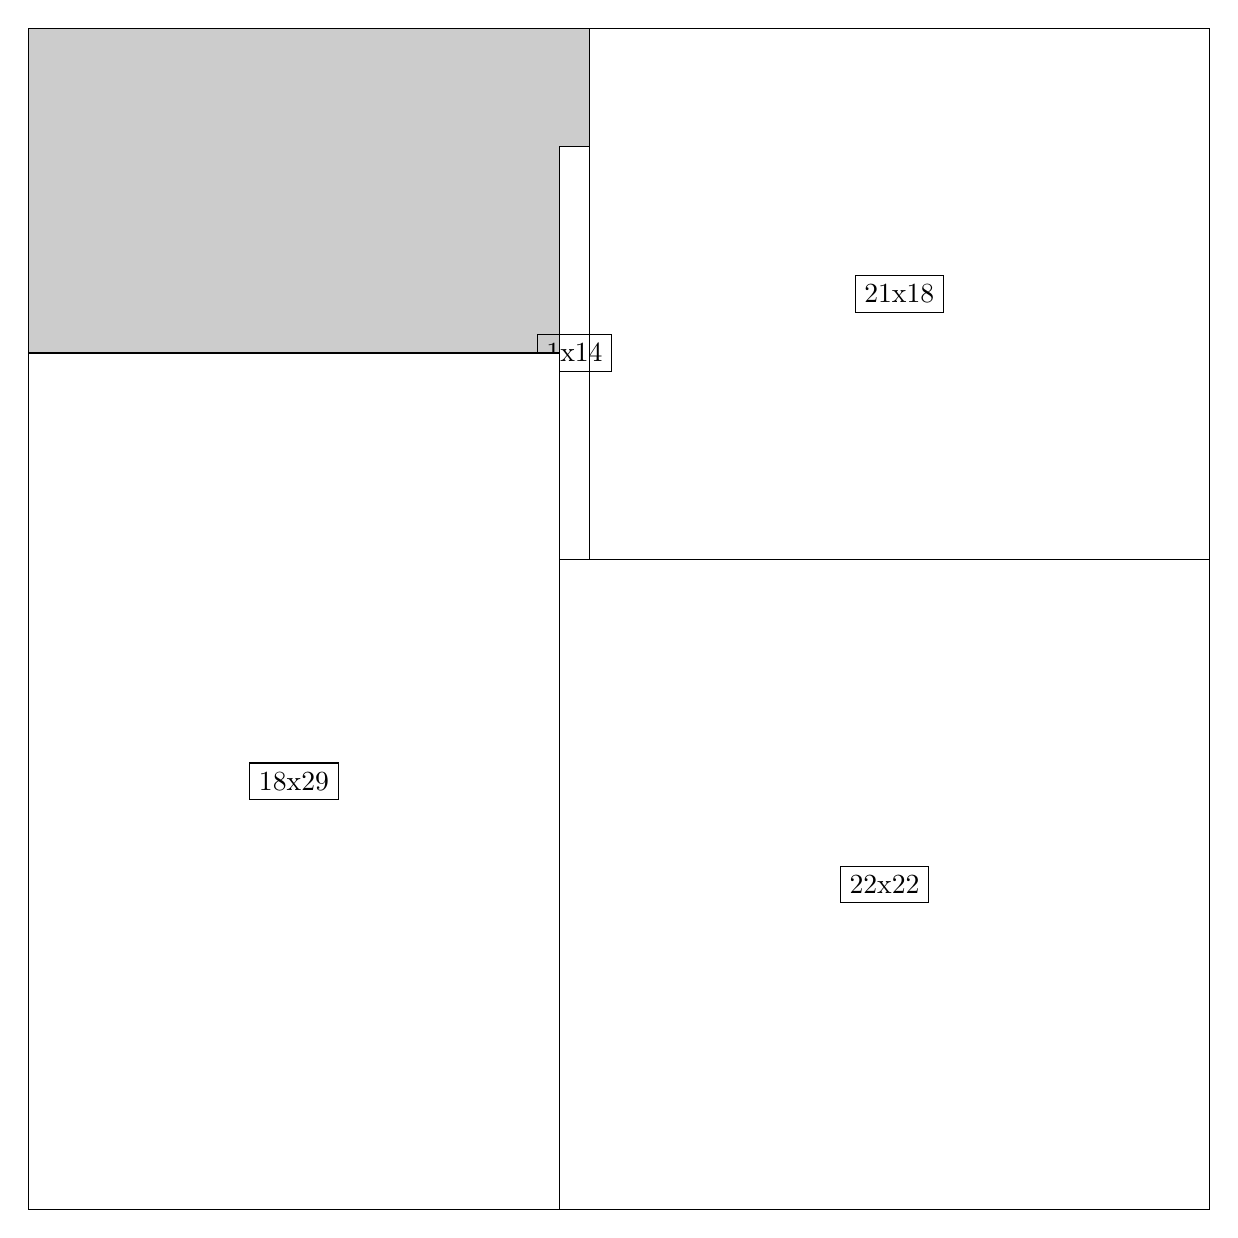
\begin{tikzpicture}[shorten >=1pt,scale=1.0,every node/.style={scale=1.0},->]
\tikzstyle{vertex}=[circle,fill=black!25,minimum size=14pt,inner sep=0pt]
\filldraw[fill=gray!40!white, draw=black] (0,0) rectangle (15.0,15.0);
\foreach \name/\x/\y/\w/\h in {22x22/6.75/0.0/8.25/8.25,21x18/7.125/8.25/7.875/6.75,1x14/6.75/8.25/0.375/5.25,18x29/0.0/0.0/6.75/10.875}
\filldraw[fill=white!40!white, draw=black] (\x,\y) rectangle node[draw] (\name) {\name} ++(\w,\h);
\end{tikzpicture}


w =22 , h =22 , x =18 , y =0 , v =484
\par
w =21 , h =18 , x =19 , y =22 , v =378
\par
w =1 , h =14 , x =18 , y =22 , v =14
\par
w =18 , h =29 , x =0 , y =0 , v =522
\par
\newpage


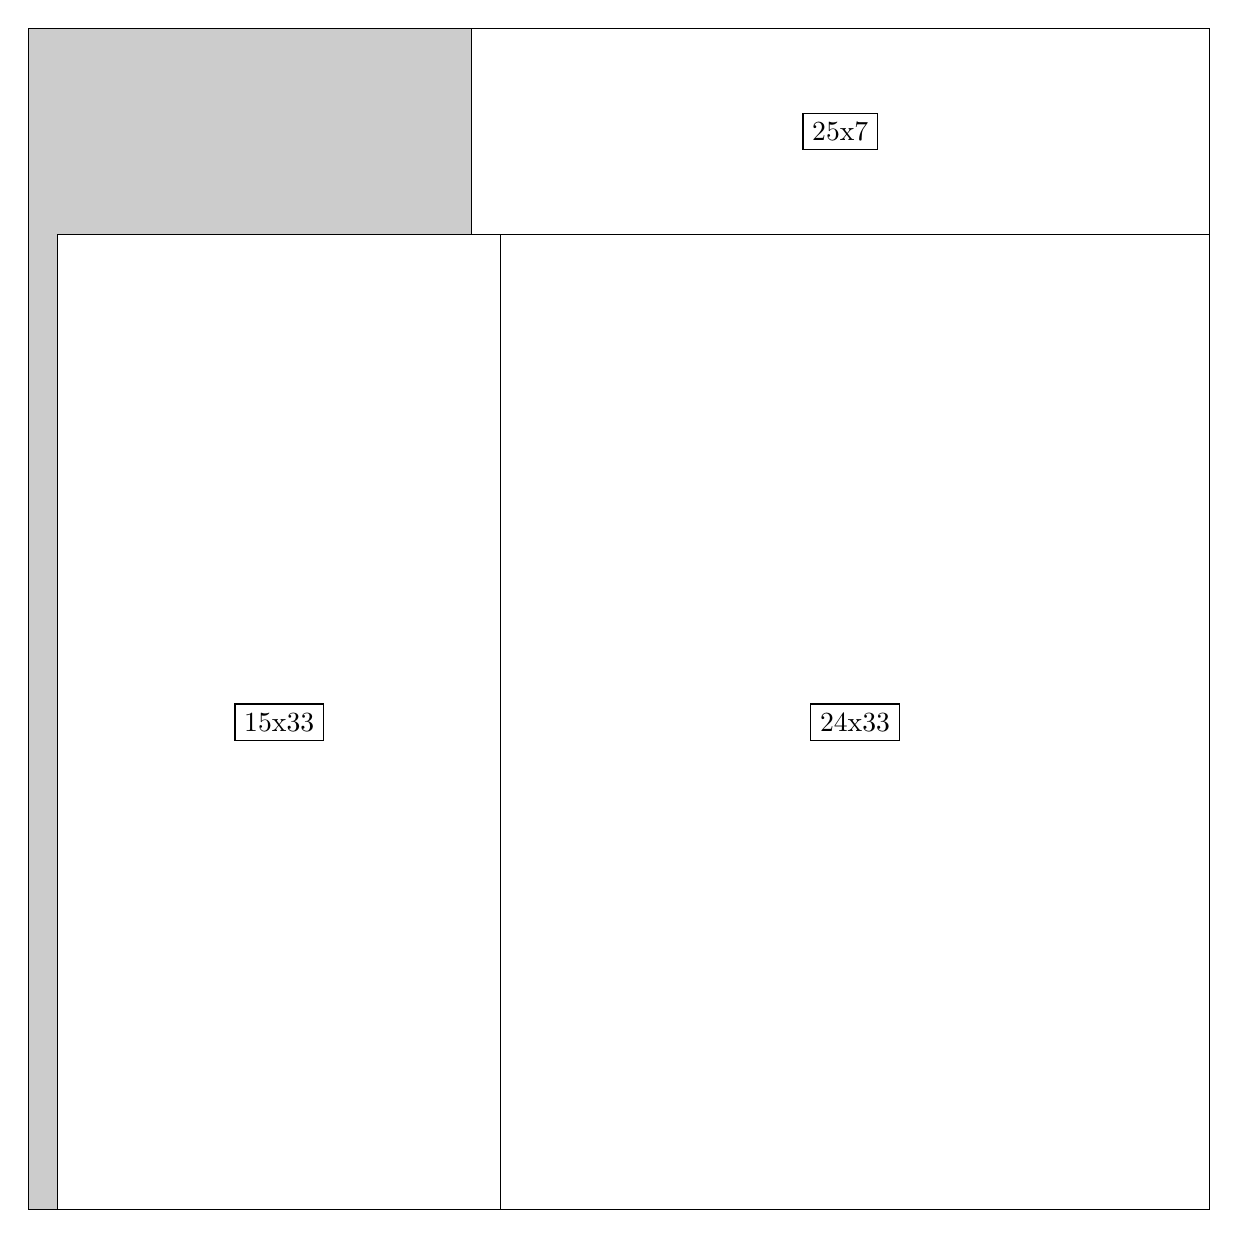
\begin{tikzpicture}[shorten >=1pt,scale=1.0,every node/.style={scale=1.0},->]
\tikzstyle{vertex}=[circle,fill=black!25,minimum size=14pt,inner sep=0pt]
\filldraw[fill=gray!40!white, draw=black] (0,0) rectangle (15.0,15.0);
\foreach \name/\x/\y/\w/\h in {24x33/6.0/0.0/9.0/12.375,15x33/0.375/0.0/5.625/12.375,25x7/5.625/12.375/9.375/2.625}
\filldraw[fill=white!40!white, draw=black] (\x,\y) rectangle node[draw] (\name) {\name} ++(\w,\h);
\end{tikzpicture}


w =24 , h =33 , x =16 , y =0 , v =792
\par
w =15 , h =33 , x =1 , y =0 , v =495
\par
w =25 , h =7 , x =15 , y =33 , v =175
\par
\newpage


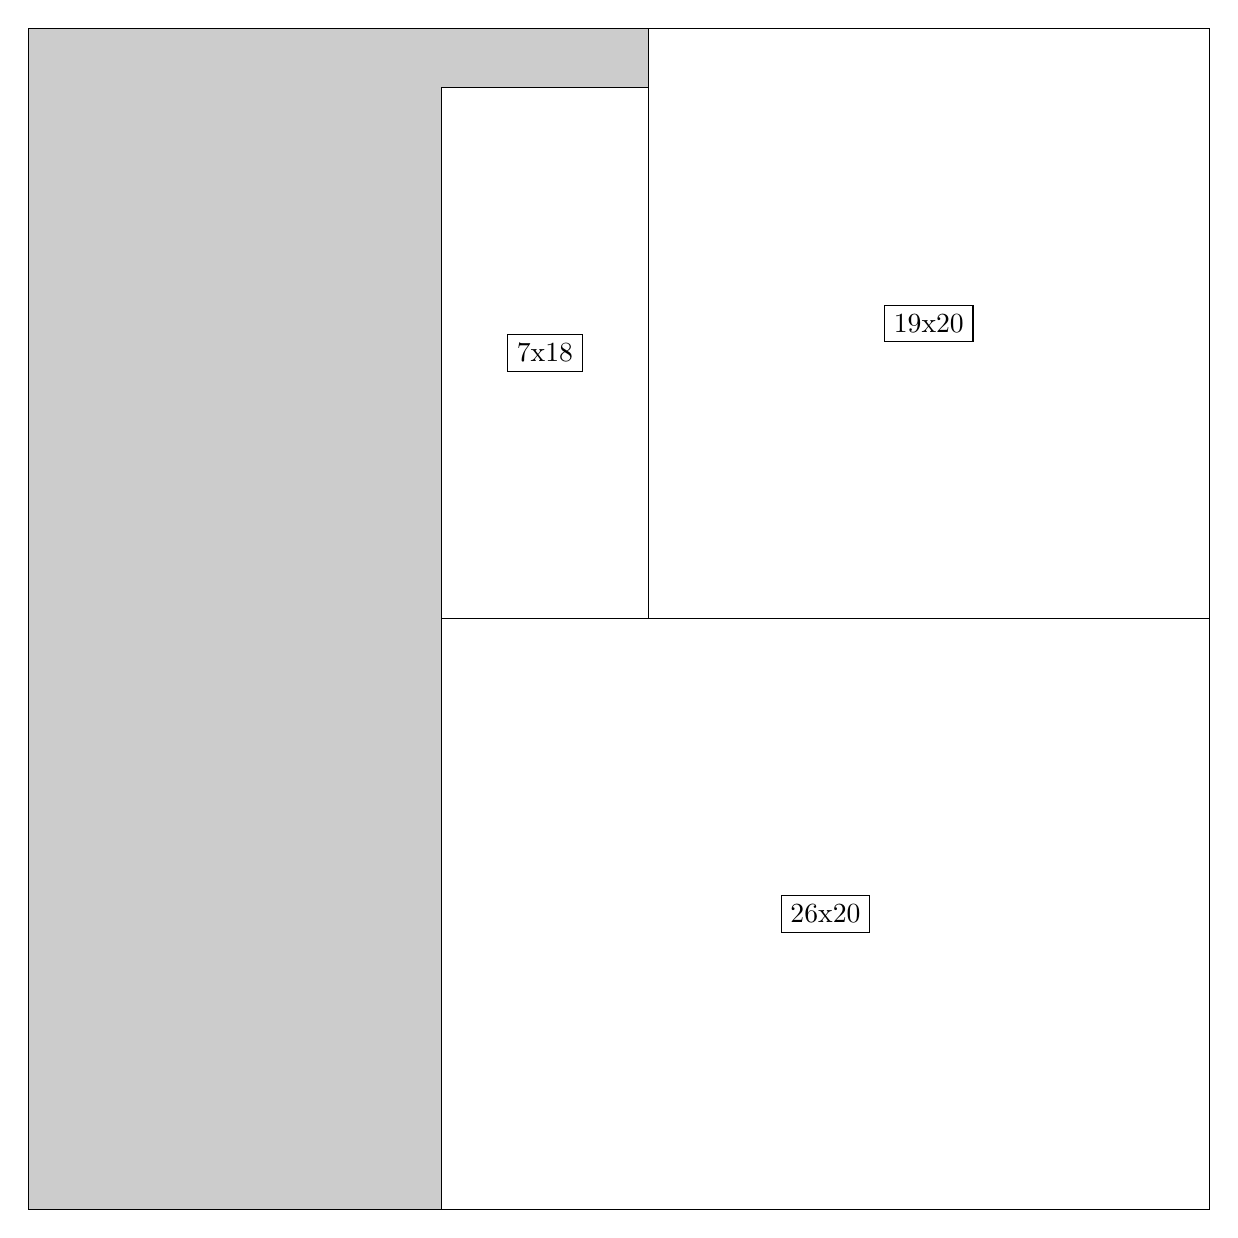
\begin{tikzpicture}[shorten >=1pt,scale=1.0,every node/.style={scale=1.0},->]
\tikzstyle{vertex}=[circle,fill=black!25,minimum size=14pt,inner sep=0pt]
\filldraw[fill=gray!40!white, draw=black] (0,0) rectangle (15.0,15.0);
\foreach \name/\x/\y/\w/\h in {26x20/5.25/0.0/9.75/7.5,19x20/7.875/7.5/7.125/7.5,7x18/5.25/7.5/2.625/6.75}
\filldraw[fill=white!40!white, draw=black] (\x,\y) rectangle node[draw] (\name) {\name} ++(\w,\h);
\end{tikzpicture}


w =26 , h =20 , x =14 , y =0 , v =520
\par
w =19 , h =20 , x =21 , y =20 , v =380
\par
w =7 , h =18 , x =14 , y =20 , v =126
\par
\newpage


\begin{tikzpicture}[shorten >=1pt,scale=1.0,every node/.style={scale=1.0},->]
\tikzstyle{vertex}=[circle,fill=black!25,minimum size=14pt,inner sep=0pt]
\filldraw[fill=gray!40!white, draw=black] (0,0) rectangle (15.0,15.0);
\foreach \name/\x/\y/\w/\h in {34x14/2.25/0.0/12.75/5.25,6x14/0.0/0.0/2.25/5.25,27x26/4.875/5.25/10.125/9.75,11x25/0.75/5.25/4.125/9.375,2x24/0.0/5.25/0.75/9.0,12x1/0.375/14.625/4.5/0.375}
\filldraw[fill=white!40!white, draw=black] (\x,\y) rectangle node[draw] (\name) {\name} ++(\w,\h);
\end{tikzpicture}


w =34 , h =14 , x =6 , y =0 , v =476
\par
w =6 , h =14 , x =0 , y =0 , v =84
\par
w =27 , h =26 , x =13 , y =14 , v =702
\par
w =11 , h =25 , x =2 , y =14 , v =275
\par
w =2 , h =24 , x =0 , y =14 , v =48
\par
w =12 , h =1 , x =1 , y =39 , v =12
\par
\newpage


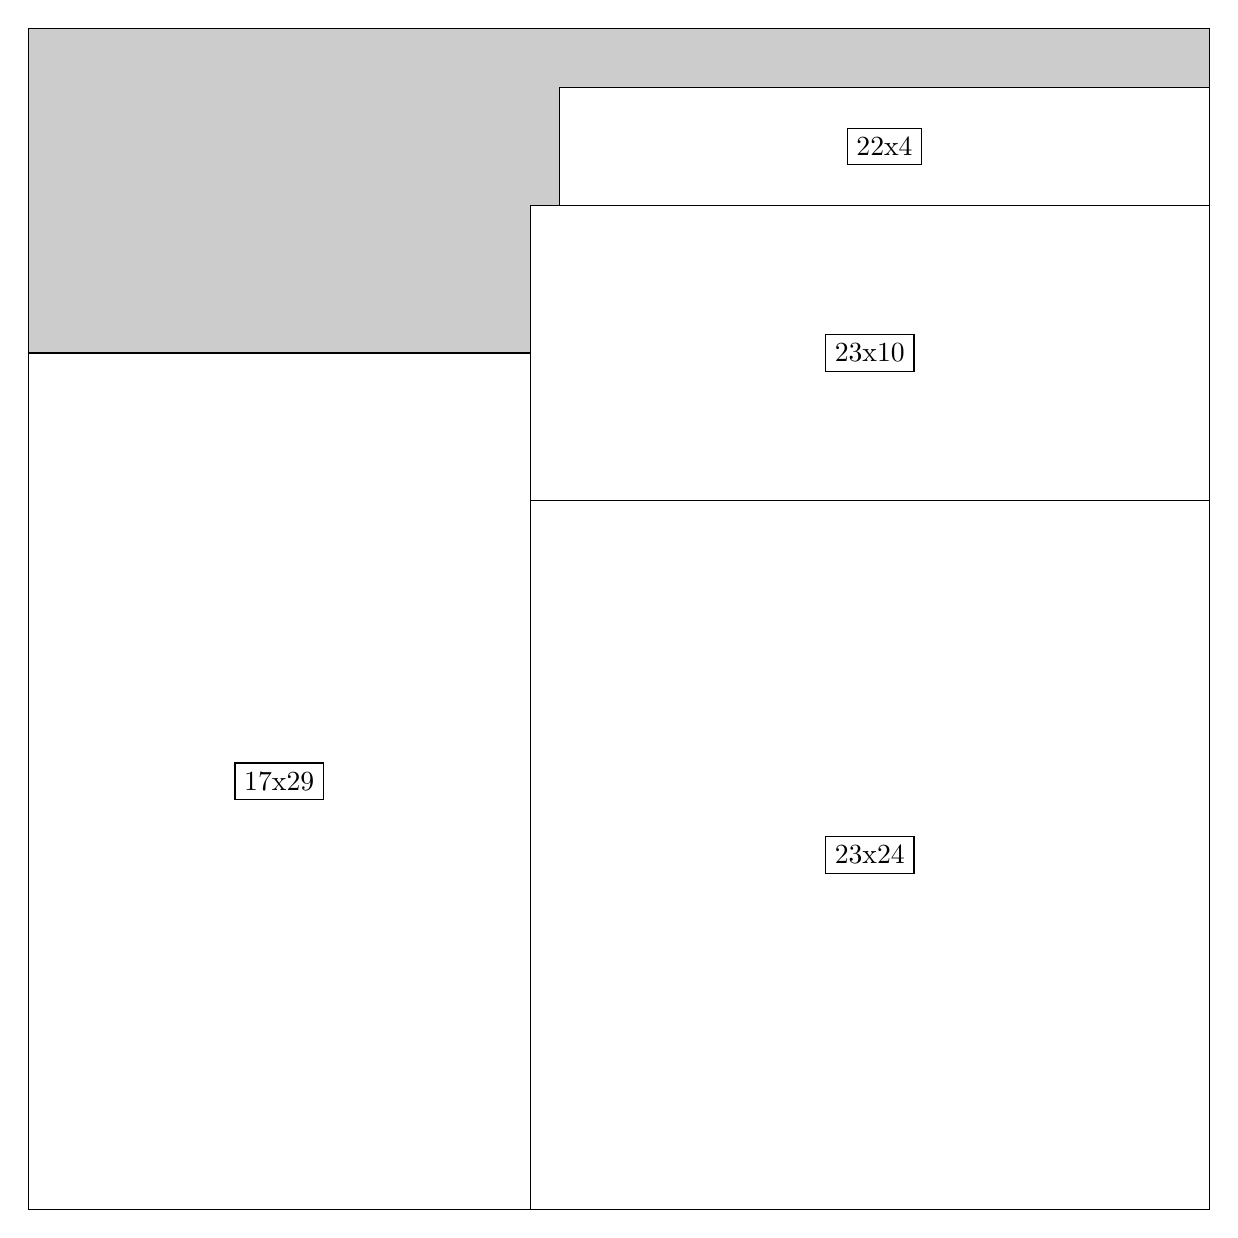
\begin{tikzpicture}[shorten >=1pt,scale=1.0,every node/.style={scale=1.0},->]
\tikzstyle{vertex}=[circle,fill=black!25,minimum size=14pt,inner sep=0pt]
\filldraw[fill=gray!40!white, draw=black] (0,0) rectangle (15.0,15.0);
\foreach \name/\x/\y/\w/\h in {23x24/6.375/0.0/8.625/9.0,23x10/6.375/9.0/8.625/3.75,22x4/6.75/12.75/8.25/1.5,17x29/0.0/0.0/6.375/10.875}
\filldraw[fill=white!40!white, draw=black] (\x,\y) rectangle node[draw] (\name) {\name} ++(\w,\h);
\end{tikzpicture}


w =23 , h =24 , x =17 , y =0 , v =552
\par
w =23 , h =10 , x =17 , y =24 , v =230
\par
w =22 , h =4 , x =18 , y =34 , v =88
\par
w =17 , h =29 , x =0 , y =0 , v =493
\par
\newpage


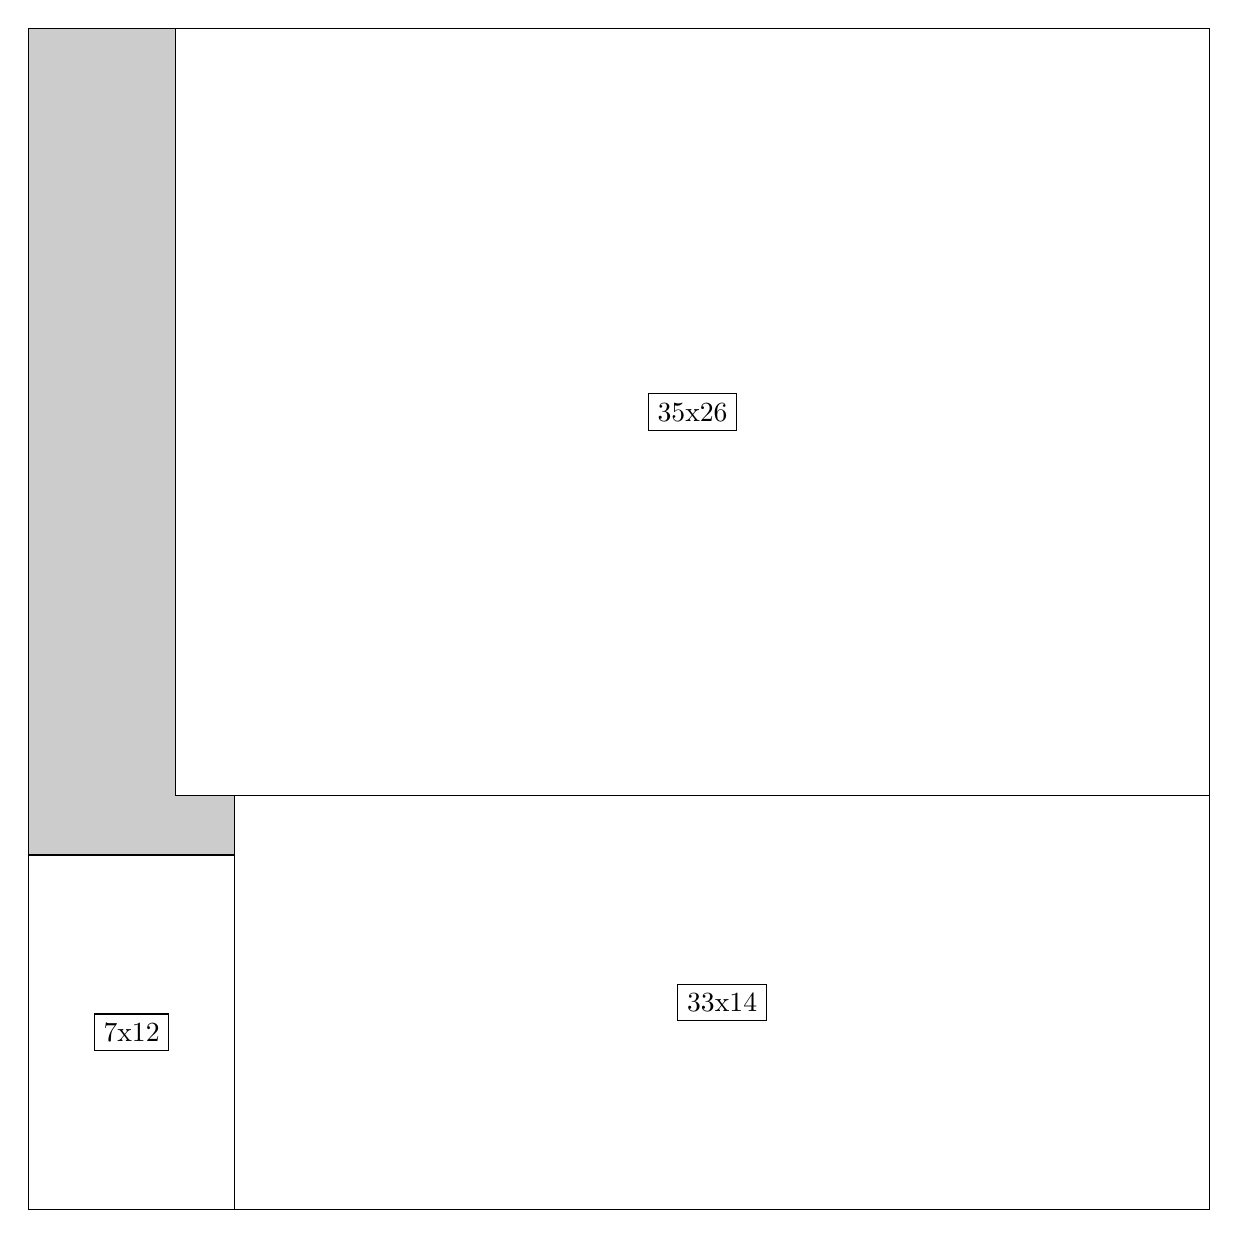
\begin{tikzpicture}[shorten >=1pt,scale=1.0,every node/.style={scale=1.0},->]
\tikzstyle{vertex}=[circle,fill=black!25,minimum size=14pt,inner sep=0pt]
\filldraw[fill=gray!40!white, draw=black] (0,0) rectangle (15.0,15.0);
\foreach \name/\x/\y/\w/\h in {33x14/2.625/0.0/12.375/5.25,7x12/0.0/0.0/2.625/4.5,35x26/1.875/5.25/13.125/9.75}
\filldraw[fill=white!40!white, draw=black] (\x,\y) rectangle node[draw] (\name) {\name} ++(\w,\h);
\end{tikzpicture}


w =33 , h =14 , x =7 , y =0 , v =462
\par
w =7 , h =12 , x =0 , y =0 , v =84
\par
w =35 , h =26 , x =5 , y =14 , v =910
\par
\newpage


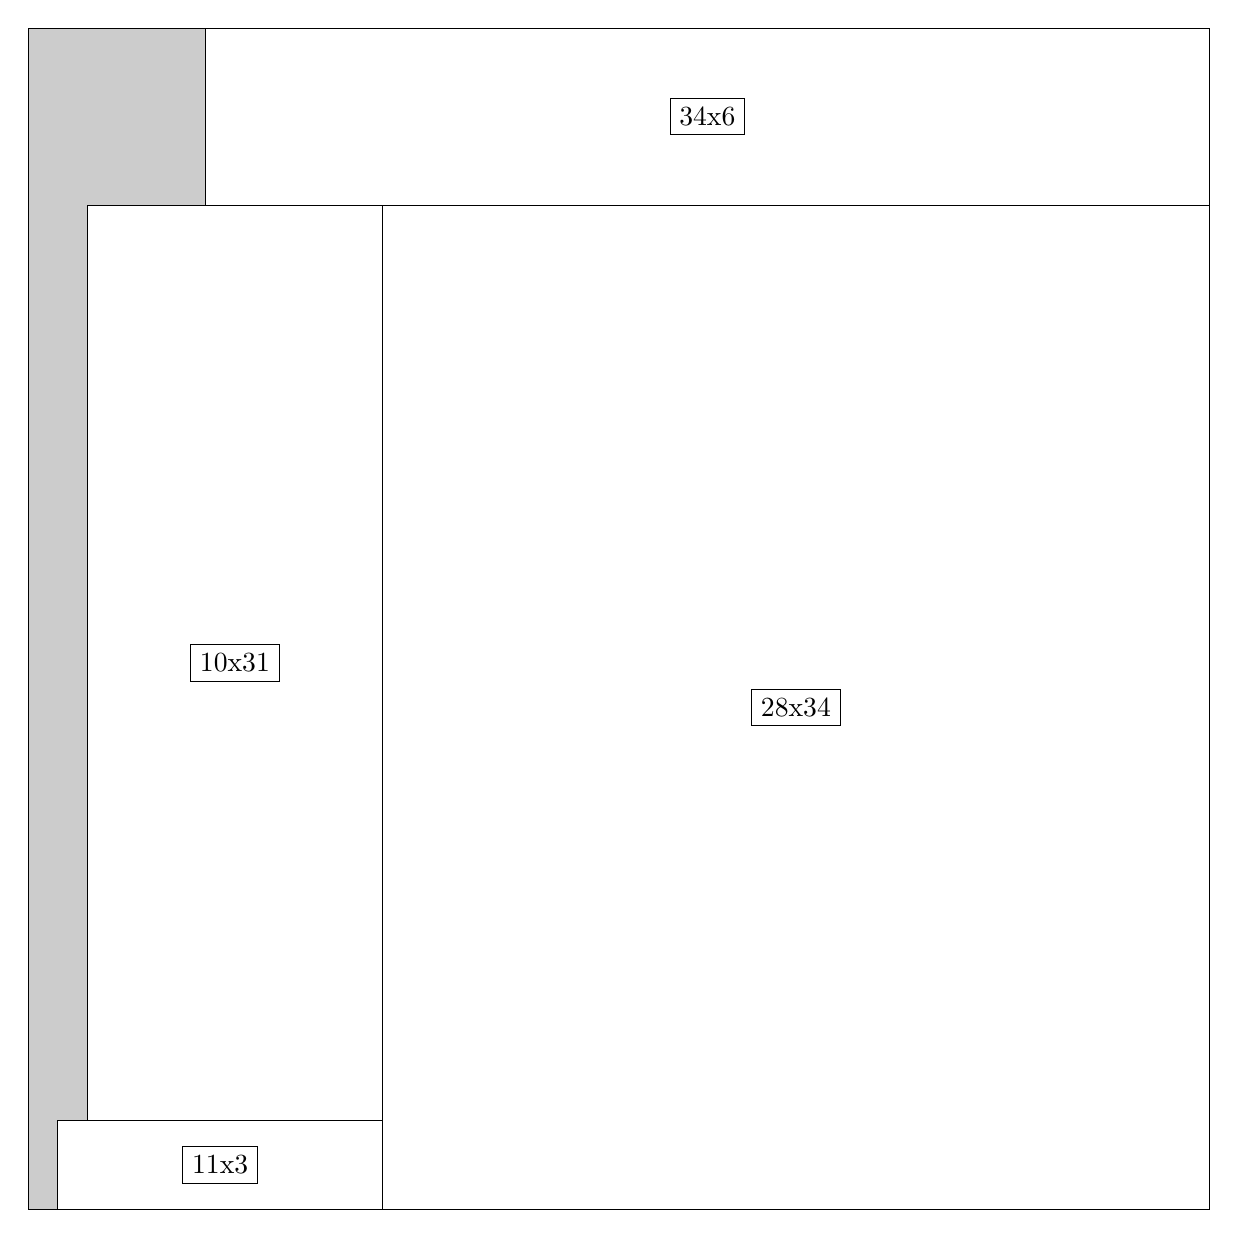
\begin{tikzpicture}[shorten >=1pt,scale=1.0,every node/.style={scale=1.0},->]
\tikzstyle{vertex}=[circle,fill=black!25,minimum size=14pt,inner sep=0pt]
\filldraw[fill=gray!40!white, draw=black] (0,0) rectangle (15.0,15.0);
\foreach \name/\x/\y/\w/\h in {28x34/4.5/0.0/10.5/12.75,11x3/0.375/0.0/4.125/1.125,10x31/0.75/1.125/3.75/11.625,34x6/2.25/12.75/12.75/2.25}
\filldraw[fill=white!40!white, draw=black] (\x,\y) rectangle node[draw] (\name) {\name} ++(\w,\h);
\end{tikzpicture}


w =28 , h =34 , x =12 , y =0 , v =952
\par
w =11 , h =3 , x =1 , y =0 , v =33
\par
w =10 , h =31 , x =2 , y =3 , v =310
\par
w =34 , h =6 , x =6 , y =34 , v =204
\par
\newpage


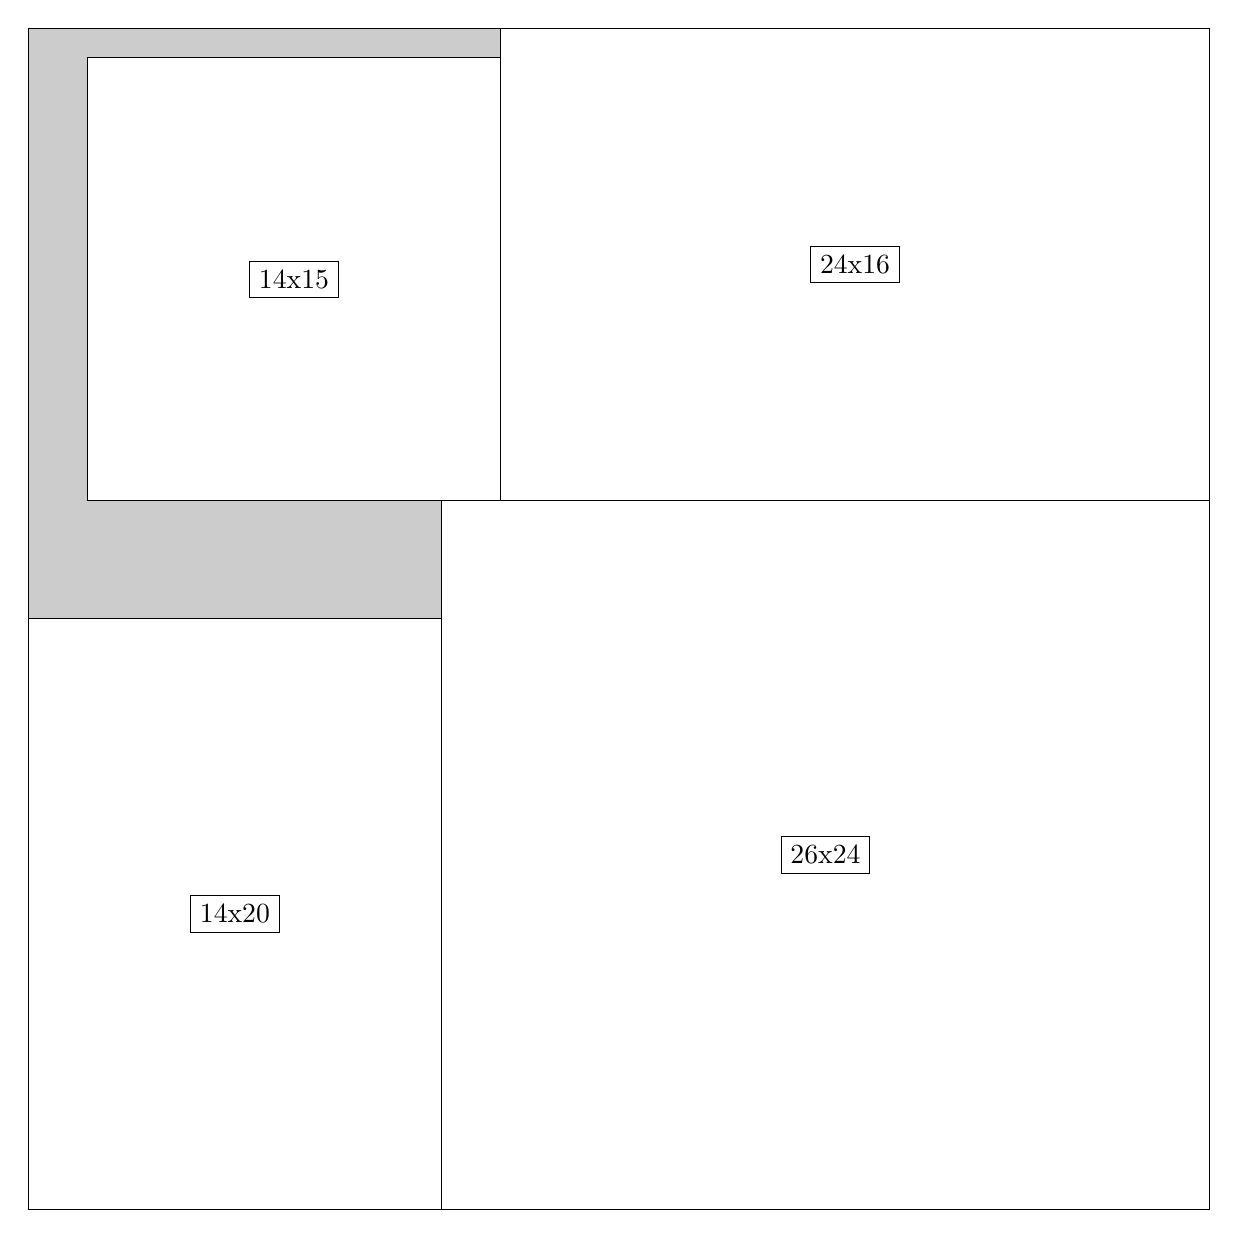
\begin{tikzpicture}[shorten >=1pt,scale=1.0,every node/.style={scale=1.0},->]
\tikzstyle{vertex}=[circle,fill=black!25,minimum size=14pt,inner sep=0pt]
\filldraw[fill=gray!40!white, draw=black] (0,0) rectangle (15.0,15.0);
\foreach \name/\x/\y/\w/\h in {26x24/5.25/0.0/9.75/9.0,14x20/0.0/0.0/5.25/7.5,24x16/6.0/9.0/9.0/6.0,14x15/0.75/9.0/5.25/5.625}
\filldraw[fill=white!40!white, draw=black] (\x,\y) rectangle node[draw] (\name) {\name} ++(\w,\h);
\end{tikzpicture}


w =26 , h =24 , x =14 , y =0 , v =624
\par
w =14 , h =20 , x =0 , y =0 , v =280
\par
w =24 , h =16 , x =16 , y =24 , v =384
\par
w =14 , h =15 , x =2 , y =24 , v =210
\par
\newpage


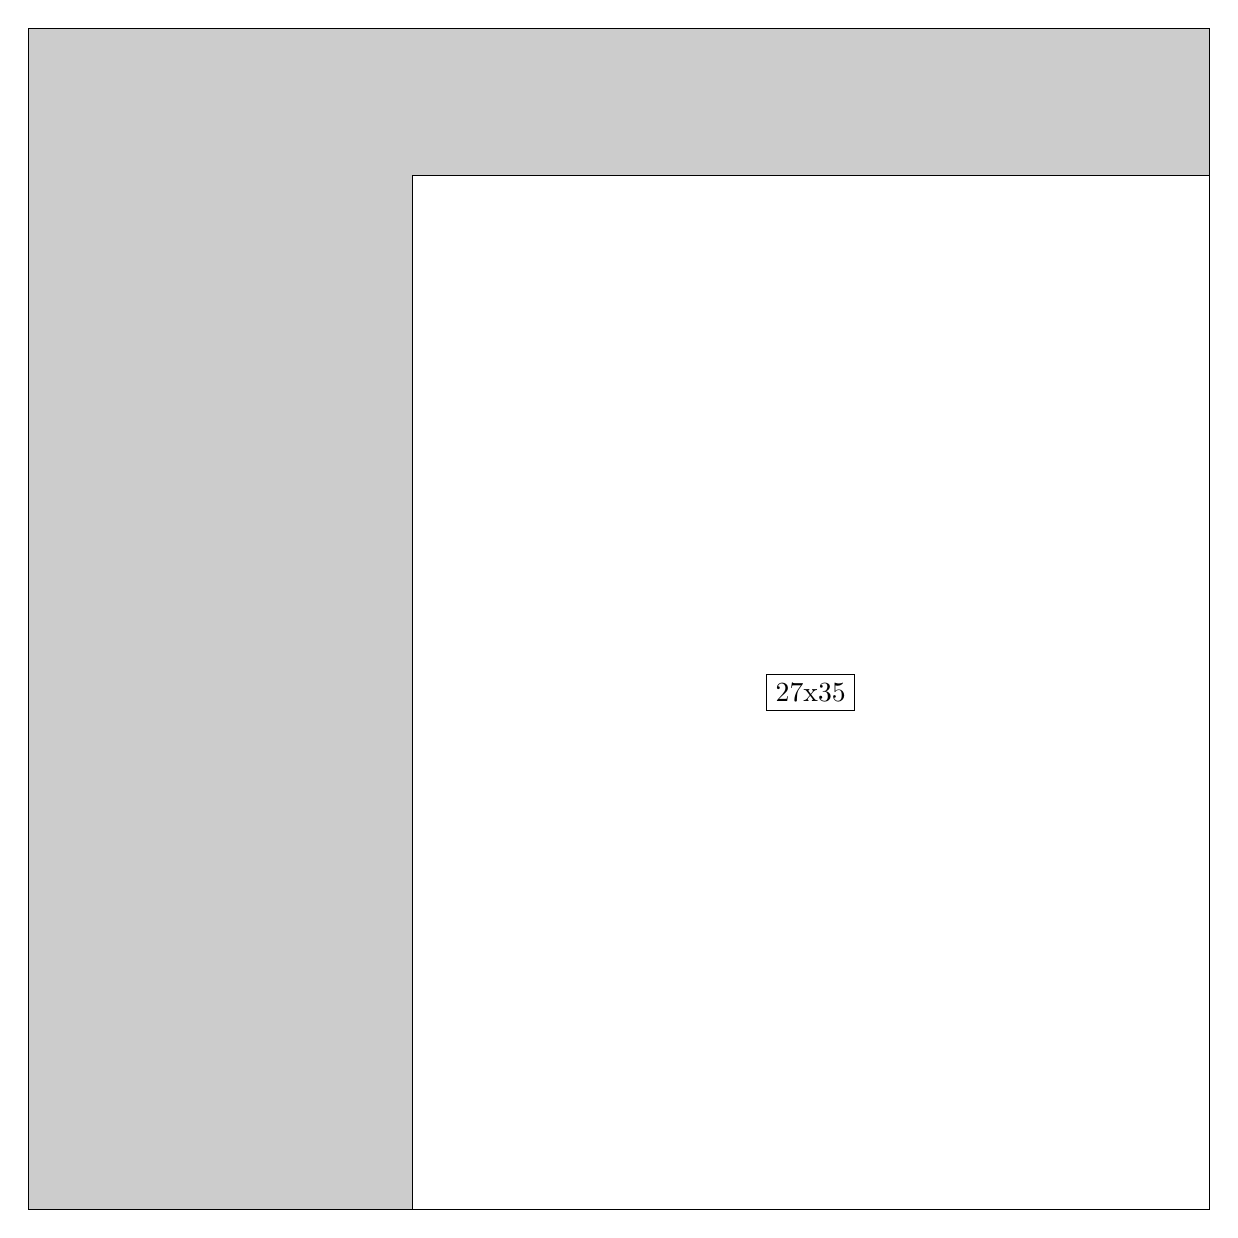
\begin{tikzpicture}[shorten >=1pt,scale=1.0,every node/.style={scale=1.0},->]
\tikzstyle{vertex}=[circle,fill=black!25,minimum size=14pt,inner sep=0pt]
\filldraw[fill=gray!40!white, draw=black] (0,0) rectangle (15.0,15.0);
\foreach \name/\x/\y/\w/\h in {27x35/4.875/0.0/10.125/13.125}
\filldraw[fill=white!40!white, draw=black] (\x,\y) rectangle node[draw] (\name) {\name} ++(\w,\h);
\end{tikzpicture}


w =27 , h =35 , x =13 , y =0 , v =945
\par
\newpage


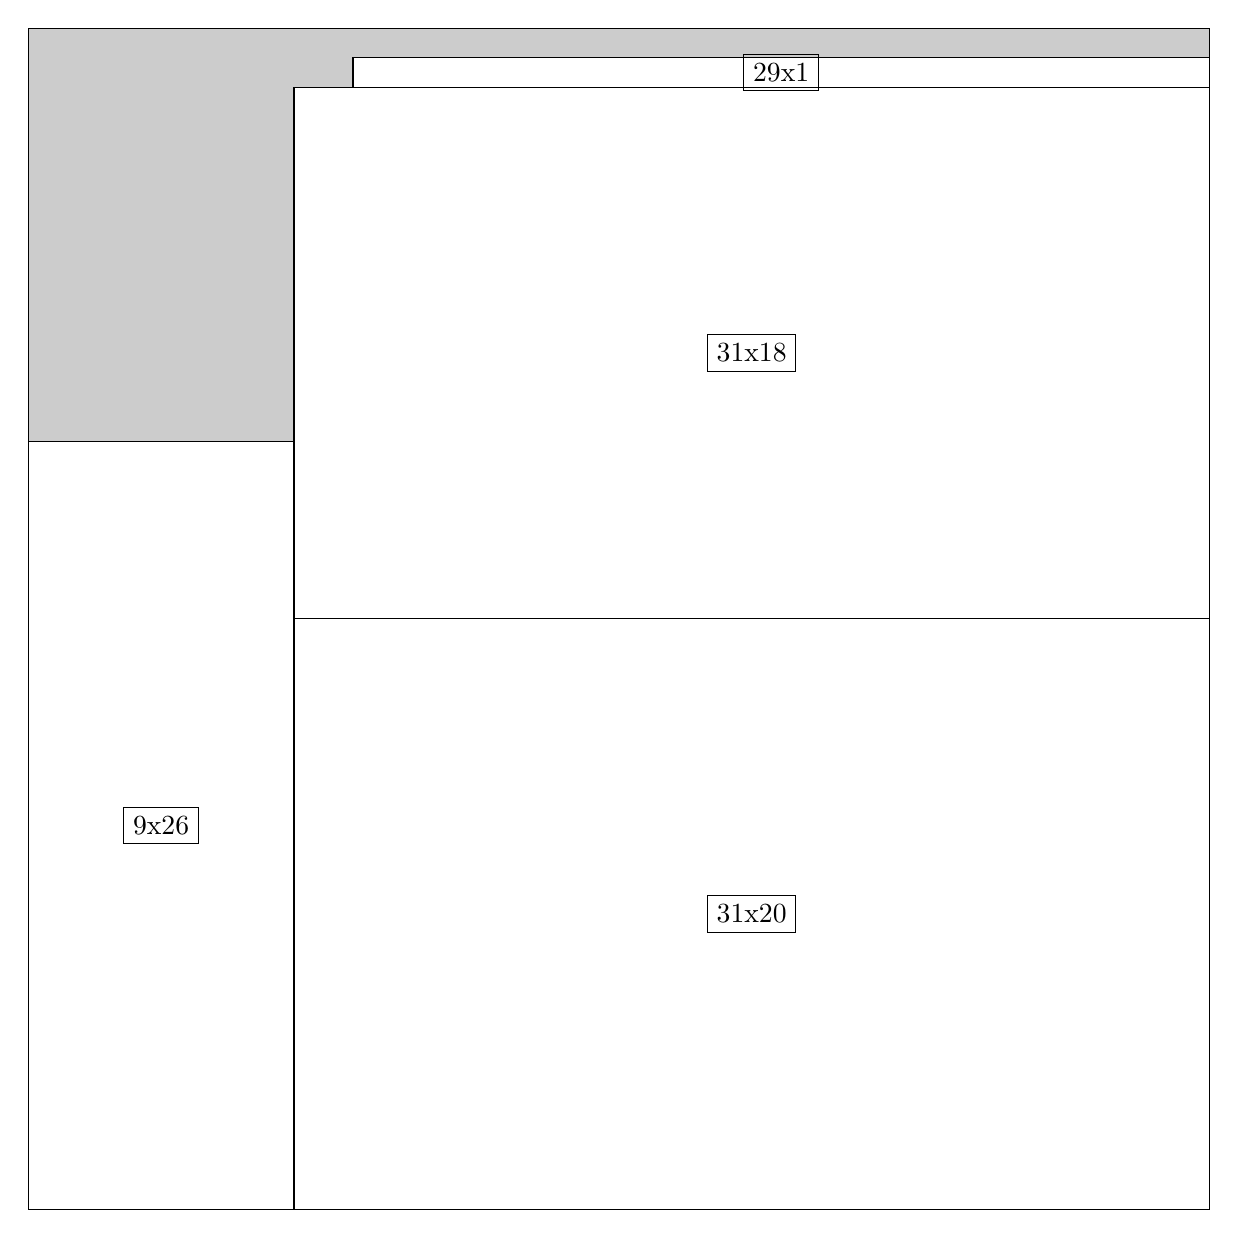
\begin{tikzpicture}[shorten >=1pt,scale=1.0,every node/.style={scale=1.0},->]
\tikzstyle{vertex}=[circle,fill=black!25,minimum size=14pt,inner sep=0pt]
\filldraw[fill=gray!40!white, draw=black] (0,0) rectangle (15.0,15.0);
\foreach \name/\x/\y/\w/\h in {31x20/3.375/0.0/11.625/7.5,31x18/3.375/7.5/11.625/6.75,29x1/4.125/14.25/10.875/0.375,9x26/0.0/0.0/3.375/9.75}
\filldraw[fill=white!40!white, draw=black] (\x,\y) rectangle node[draw] (\name) {\name} ++(\w,\h);
\end{tikzpicture}


w =31 , h =20 , x =9 , y =0 , v =620
\par
w =31 , h =18 , x =9 , y =20 , v =558
\par
w =29 , h =1 , x =11 , y =38 , v =29
\par
w =9 , h =26 , x =0 , y =0 , v =234
\par
\newpage


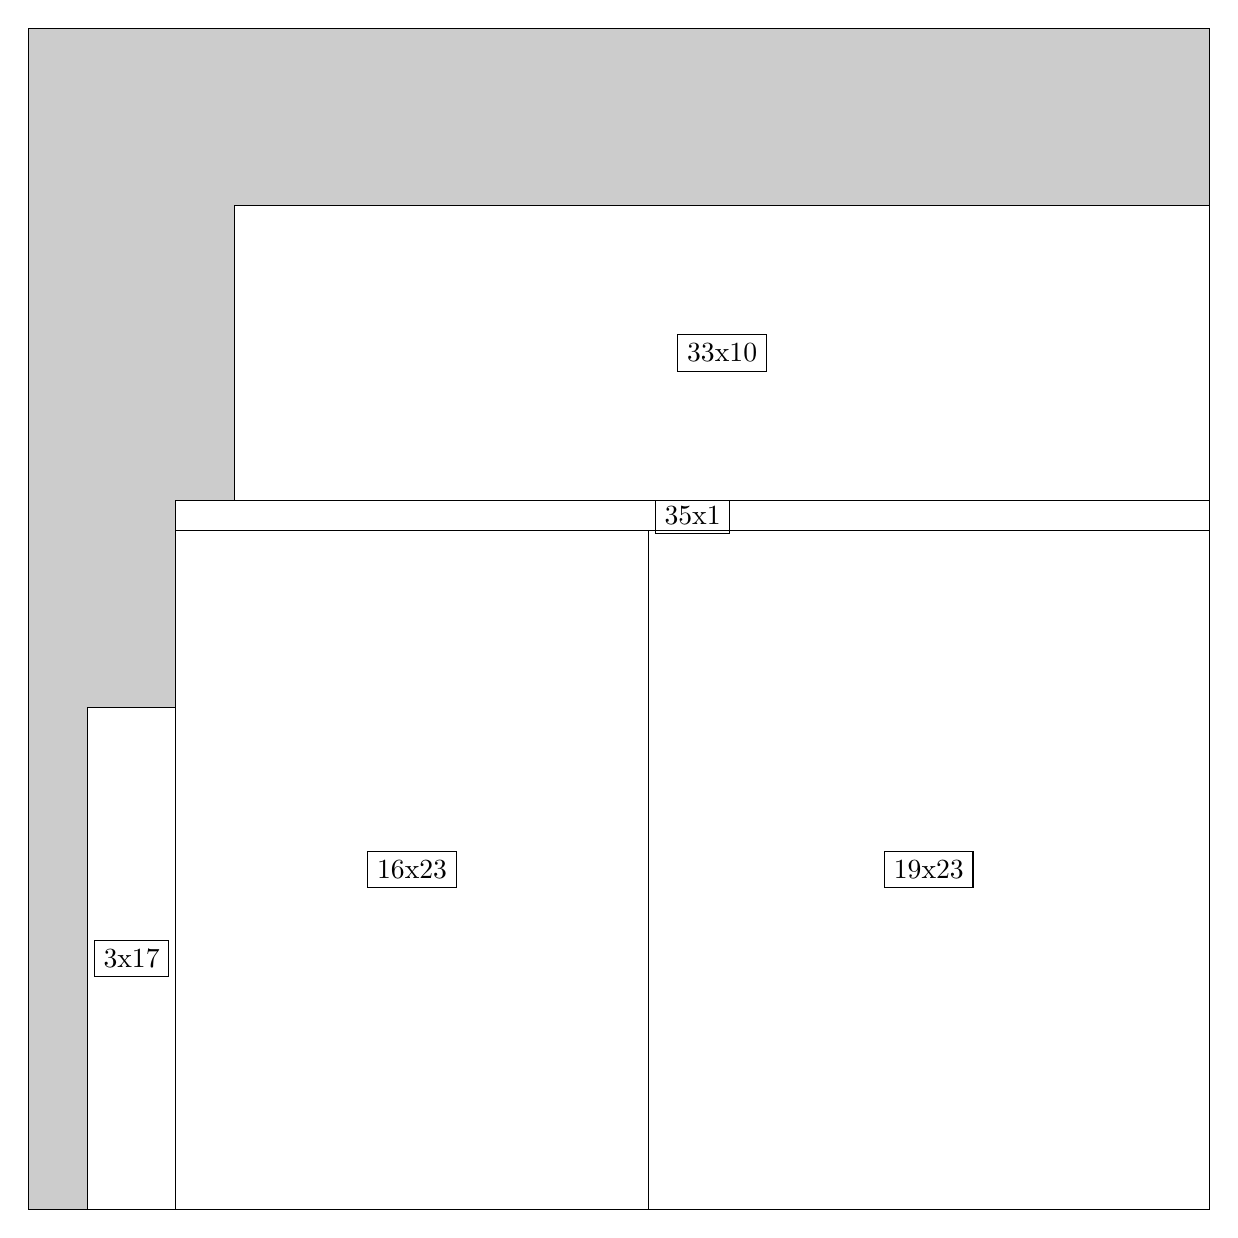
\begin{tikzpicture}[shorten >=1pt,scale=1.0,every node/.style={scale=1.0},->]
\tikzstyle{vertex}=[circle,fill=black!25,minimum size=14pt,inner sep=0pt]
\filldraw[fill=gray!40!white, draw=black] (0,0) rectangle (15.0,15.0);
\foreach \name/\x/\y/\w/\h in {19x23/7.875/0.0/7.125/8.625,16x23/1.875/0.0/6.0/8.625,3x17/0.75/0.0/1.125/6.375,35x1/1.875/8.625/13.125/0.375,33x10/2.625/9.0/12.375/3.75}
\filldraw[fill=white!40!white, draw=black] (\x,\y) rectangle node[draw] (\name) {\name} ++(\w,\h);
\end{tikzpicture}


w =19 , h =23 , x =21 , y =0 , v =437
\par
w =16 , h =23 , x =5 , y =0 , v =368
\par
w =3 , h =17 , x =2 , y =0 , v =51
\par
w =35 , h =1 , x =5 , y =23 , v =35
\par
w =33 , h =10 , x =7 , y =24 , v =330
\par
\newpage


\end{document}